\documentclass[11pt,a4paper]{article}

% Codificação e idioma
\usepackage[utf8]{inputenc}
\usepackage[T1]{fontenc}
\usepackage[brazil]{babel}

% Fonte: para usar fonte sem serifa como padrão
\usepackage{helvet}
\renewcommand{\familydefault}{\sfdefault}

% Margens de 2cm em todos os lados
\usepackage[a4paper, margin=2cm]{geometry}

% Espaçamento 1,5 entre linhas
\usepackage{setspace}
\onehalfspacing

% Configuração para quebras de linha naturais
\usepackage{parskip}
\setlength{\parskip}{0.3\baselineskip}
\setlength{\parindent}{0pt}

% Pacotes para gráficos, tabelas e links (se necessário)
\usepackage{graphicx}
\usepackage{float}
\usepackage{amsmath,amssymb}
\usepackage{hyperref}
\usepackage{subcaption}
\usepackage{xcolor}
\usepackage{listings}

\lstset{
    inputencoding=utf8,
    extendedchars=true,
    literate=
        {á}{{\'a}}1 {à}{{\`a}}1 {â}{{\^a}}1 {ã}{{\~a}}1 {Á}{{\'A}}1 {À}{{\`A}}1 {Â}{{\^A}}1 {Ã}{{\~A}}1
        {é}{{\'e}}1 {è}{{\`e}}1 {ê}{{\^e}}1 {É}{{\'E}}1 {È}{{\`E}}1 {Ê}{{\^E}}1
        {í}{{\'i}}1 {ì}{{\`i}}1 {î}{{\^i}}1 {Í}{{\'I}}1 {Ì}{{\`I}}1 {Î}{{\^I}}1
        {ó}{{\'o}}1 {ò}{{\`o}}1 {ô}{{\^o}}1 {õ}{{\~o}}1 {Ó}{{\'O}}1 {Ò}{{\`O}}1 {Ô}{{\^O}}1 {Õ}{{\~O}}1
        {ú}{{\'u}}1 {ù}{{\`u}}1 {û}{{\^u}}1 {Ú}{{\'U}}1 {Ù}{{\`U}}1 {Û}{{\^U}}1
        {ç}{{\c c}}1 {Ç}{{\c C}}1
        {–}{-}1 {—}{--}1 {×}{x}1 {ō}{o}1,
    basicstyle=\ttfamily\small,
    keywordstyle=\color{blue},
    stringstyle=\color{red!80!black},
    commentstyle=\color{green!60!black},
    showstringspaces=false,
    breaklines=true,
    frame=single,
    framerule=0pt,
    backgroundcolor=\color{black!5},
    numbers=left,
    numberstyle=\tiny\color{gray}
}

\hypersetup{
    colorlinks=true,
    linkcolor=blue,
    urlcolor=blue
}

% Informações do título e autores
\title{A arte nos dados: \\ Inferência estatística sobre popularidade, temporalidade e atributos físicos de obras do Metropolitan Museum of Art}
\author{
  Beatriz Reis Repette \\
  Diego Martins Meditsch \\
  Pedro Henrique Gimenez \\
  Tom Pereira Hunt \\
  \\
  Universidade Federal de Santa Catarina \\
  Florianópolis, 2025
}
\date{}

\begin{document}

\maketitle

% Seção: Introdução e Objetivos
\section{Introdução e Objetivos}
Este trabalho dá continuidade à análise do acervo público do Metropolitan Museum of Art (MET), com foco em pinturas e esculturas. O objetivo principal é aplicar métodos estatísticos inferenciais sobre variáveis selecionadas no Trabalho 1, a fim de validar relações entre materiais, culturas, popularidade e temporalidade.

Neste estudo, formulamos e testamos hipóteses sobre média, proporção, correlação e regressão. A investigação busca traçar paralelos interessantes entre a popularidade atual das obras e suas características físicas e temáticas.

Os dados que utilizamos foram obtidos por meio de uma iniciativa do próprio museu, que os disponibiliza publicamente. Eles foram acessados em 12 de março de 2025, no GitHub, onde foram disponibilizados gratuitamente pelo próprio museu e atualizados pela última vez no dia 17 de junho de 2023 \cite{ref1}.

A partir da apresentação dos dados coletados, buscamos investigar quatro hipóteses:
\begin{enumerate}
    \item \textbf{Hipótese sobre média:} \\H\textsubscript{0}: A média da área das pinturas destacadas é igual à das não destacadas.
    \item \textbf{Hipótese sobre proporção:} \\H\textsubscript{0}: A proporção de obras com tema religioso entre os destaques é igual à dos não destacados.
    \item \textbf{Hipótese sobre correlação:} \\H\textsubscript{0}: Não há correlação entre o ano da obra e a sua popularidade.
    \item \textbf{Hipótese sobre regressão linear:} \\H\textsubscript{0}: O ano de confecção de uma escultura não influencia seu volume.
\end{enumerate}
Dessa forma, será possível tirar as devidas conclusões conforme os resultados.

% Seção: Materiais e Métodos
\section{Materiais e Métodos}
Para nossa análise, selecionamos as variáveis que caracterizam os principais atributos das obras: ano de confecção, dimensões físicas, temática e se a obra é destaque no acervo. O conjunto de dados foi extraído do repositório público do MET no GitHub \cite{ref1}. 
Das, aproximadamente, 480 mil peças originais, restringimos a análise apenas a pinturas e esculturas, obtendo 15.124 obras.

Em relação às variáveis escolhidas, seus nomes no banco de dados (entre parênteses, em itálico), suas classificações, descrições, motivo de escolha e possíveis observações, seguem:

\subsection*{Ano do objeto (\textit{Object Begin Date})}
\begin{itemize}
    \item \textbf{Classificação:} Variável quantitativa contínua.
    \item \textbf{Descrição:} Ano de criação do objeto, ou aproximado, se não houver registro exato. Extraído diretamente do banco de dados (não foi nossa aproximação).
    \item \textbf{Motivo de escolha:} Estes dados contribuirão para a validação das hipóteses 3 e 4.
\end{itemize}

\subsection*{Dimensões (\textit{Dimensions})}
\begin{itemize}
    \item \textbf{Classificação:} Variável quantitativa contínua.
    \item \textbf{Descrição:} Não consta no banco de dados original como número único, mas como dimensões (multiplicamos as 2 dimensões para pinturas, resultando em cm², e as 3 para esculturas, resultando em cm³).
    \item \textbf{Motivo de escolha:} Estes dados contribuirão para a validação das hipóteses 1 e 4.
    \item \textbf{Observação:} Separamos pinturas e esculturas para não misturar medidas de volume com medidas de área, o que tiraria o sentido dos dados e impossibilitaria a comparação e a análise.
\end{itemize}

\subsection*{Temáticas (\textit{Tags})}
\begin{itemize}
    \item \textbf{Classificação:} Variável qualitativa categórica.
    \item \textbf{Descrição:} Palavras que definem a temática da obra, seja de seu contexto, do que representa, de onde vem, etc.
    \item \textbf{Motivo de escolha:} Estes dados contribuirão para a validação da hipótese 2.
    \item \textbf{Observação:} Cada obra pode assumir mais de um valor de tag, mas aqui contamos cada atribuição de tag como uma entrada diferente (uma obra com 2 tags --- x e y --- conta tanto no número de ocorrências de x quanto de y).
\end{itemize}

\subsection*{É destaque (\textit{IsHighlight})}
\begin{itemize}
    \item \textbf{Classificação:} Variável qualitativa dicotômica.
    \item \textbf{Descrição:} Define se uma obra estava em destaque no momento da coleta dos dados, classificação utilizada em nossa análise para medir popularidade.
    \item \textbf{Motivo de escolha:} Estes dados contribuirão para a validação das hipóteses 1, 2 e 3.
\end{itemize}

\subsection{Procedimentos realizados}
\begin{itemize}
    \item \textbf{Limpeza e filtragem:} Selecionamos apenas registros classificados como \textit{Painting} ou \textit{Sculpture} e eliminamos itens com campos ausentes em qualquer uma das quatro variáveis-chave.
    \item \textbf{Construção de variáveis:}
        \begin{itemize}
            \item \textit{area/volume} – produto das dimensões fornecidas pelo museu (área em cm² para pinturas; volume em cm³ para esculturas).
            \item \textit{is\_sculpture} – indicador lógico que assume \texttt{TRUE} quando há três dimensões disponíveis.
        \end{itemize}
    \item \textbf{Estatística descritiva:} Cálculo de médias, desvios-padrão, proporções e respectivos intervalos de confiança (95\%).
    \item \textbf{Testes inferenciais:}
        \begin{itemize}
            \item H1: Teste t de Student.
            \item H2: Teste de proporções.
            \item H3: Correlação de Pearson.
        \end{itemize}
    \item \textbf{Modelagem para H4:} Ajuste de regressão logística com \textit{Is\_Highlight} como variável-resposta, seguida de seleção de variáveis por AIC e diagnósticos (VIF, Hosmer-Lemeshow, AUC-ROC).
\end{itemize}


% Seção: Resultados e Discussões
\section{Resultados e Discussões}

\subsection{Estatísticas Descritivas}
A base de dados utilizada neste trabalho corresponde à população total de pinturas e esculturas disponibilizadas pelo banco de dados do Metropolitan Museum of Art (MET), composta por um total de 15.124 obras, sendo 11.013 pinturas e 4.111 esculturas. A descrição do nosso banco de dados feita nesta seção leva como principais bases as variáveis do ano de realização da obra, dimensões (área para pinturas e volume para esculturas), temática (tags) e se a obra é ou não considerada um destaque na coleção.

Em relação ao \textbf{ano de criação das obras}, a média observada foi de 1377,46, com mediana em 1695 e desvio padrão de 817,07. Esses dados apontam para a presença de obras muito antigas no acervo, além de uma concentração de obras mais recentes (a mediana é relativamente alta, e existem valores muito baixos que puxam a média para baixo).

Quanto às \textbf{dimensões} físicas das obras, é possível observar uma grande dispersão tanto para pinturas quanto para esculturas. As pinturas apresentaram média de área igual a 6.472,59 cm², com mediana bem inferior (1.706,25 cm²) e desvio padrão elevado (17.567,13 cm²), o que indica a presença de outliers influenciando a média. Já as esculturas apresentaram volume médio de 167.897,29 cm³, mediana de 8.762,19 cm³ e desvio padrão extremamente elevado (1.464.062,76 cm³), o que evidencia a grande variação de tamanho dessas obras na coleção.

Ao analisar a variável de destaque, observa-se que apenas 582 das 15.124 obras (cerca de 3,85\%) recebem essa marcação, o que demonstra um critério bastante seletivo na curadoria do museu.

Por fim, ao considerar a \textbf{temática das obras}, as tags mais frequentes associadas a objetos incluem termos como \textit{Men}, \textit{Women}, \textit{Portraits} e \textit{Landscapes}, o que indica predominância de representações humanas e de cenários da natureza. De forma geral, os dados analisados mostram uma grande diversidade em termos cronológicos, físicos e temáticos.

\subsection{Testes de Hipóteses}
Dado que dispomos da população completa de pinturas e esculturas, bastaria calcular diretamente os parâmetros para responder às perguntas levantadas nas quatro hipóteses a seguir. No entanto, como o objetivo deste trabalho é aplicar métodos de inferência estatística, que são, por natureza, voltados à análise de amostras, foi necessário gerar uma amostra aleatória da população de objetos analisados, sobre a qual os testes de hipótese puderam ser realizados de forma metodologicamente adequada.

Assim, no início de cada uma das subseções seguintes, haverá uma breve discussão sobre o tamanho da amostra e a semente aleatória arbitrária utilizada para gerá-la.

\subsubsection{Média}
\textbf{H\textsubscript{0}: A média da área das pinturas destacadas é igual à das não destacadas.}

Inicialmente, foi gerada uma amostra aleatória de 1.000 pinturas, com semente fixa igual a 123, o que garante que o teste possa ser reproduzido. Após a limpeza dos dados (remoção de valores ausentes ou inválidos na variável "área"), as médias das pinturas destacadas e não destacadas foram comparadas por meio do teste t de Student para amostras independentes.

O resultado dessa primeira análise mostrou uma média de 8.983,61 cm² para as obras destacadas e 6.756,37 cm² para as não destacadas, com um p-valor igual a 0,4527. Assim, ao nível de significância de 5\% (utilizado em todas as análises desta hipótese), não rejeitamos a hipótese nula. Em outras palavras, com 95\% de confiança, não há evidências de que as médias das áreas das pinturas destacadas e não destacadas sejam significativamente diferentes.

Este é um exemplo de erro do tipo II, em que não se rejeita H\textsubscript{0} mesmo que, na população completa, a média das obras destacadas seja de fato maior. Esse tipo de erro pode ocorrer devido a diversos fatores, como alta variabilidade dos dados, tamanho amostral insuficiente, heterogeneidade interna nos grupos comparados ou, ainda, por aleatoriedade da amostragem.

Esse resultado inesperado no primeiro teste abre espaço para reflexões sobre a importância do tamanho amostral em contextos inferenciais, especialmente quando se deseja manter níveis de significância e confiança predefinidos. Podemos observar, por exemplo, que ao realizar uma segunda análise com uma amostra maior, composta por 2.000 pinturas (também com semente 123), obtemos resultados mais próximos aos populacionais. Nessa nova amostra, a média das áreas das pinturas destacadas foi de 13.494,72 cm², enquanto a das não destacadas foi de 6.175,79 cm². O p-valor obtido foi praticamente nulo, levando à rejeição da hipótese nula e indicando que há diferença estatisticamente significativa entre as médias dos dois grupos.

Com esse segundo resultado, reforçamos a noção de que testes de hipóteses podem levar a erros dependendo das condições adotadas. Ao realizar uma análise mais cuidadosa, como feito no segundo teste, com uma amostra maior, conseguimos reduzir as chances de tomar uma decisão equivocada sobre aceitar ou rejeitar uma hipótese.
	
\subsubsection{Proporção}
\textbf{H\textsubscript{0}: A proporção de obras com tema religioso entre os destaques é igual à dos não destacados.}

O código para a criação da amostra encontra-se no anexo (creating\_sample\_proportion.r), o qual gera uma amostra aleatória de 1.000 elementos de nossa população, com semente aleatória arbitrária igual a 123.

Como o critério que estamos avaliando é a proporção de obras com temáticas religiosas dentro dos destaques, foi necessária a criação de um critério que decida se uma obra tem uma tag considerada religiosa ou não. Para isso, utilizamos inteligência artificial para ajudar a filtrar as tags únicas encontradas na base de dados e separar de maneira satisfatória quais seriam religiosas. Com base nessa seleção automatizada, criamos um novo atributo qualitativo dicotômico para nossa base de dados, chamado \textit{Is\_Religious}, no qual, se um item possui uma das tags consideradas religiosas, o atributo é verdadeiro; se não possuir, é considerado falso.

Com esse novo atributo e a amostra aleatória, podemos partir para o cálculo referente à nossa hipótese. Realizamos uma contagem de dados que são religiosos, não religiosos, e o número total. Com esses valores, utilizamos a função `prop.test()` do R para realizar o teste de proporção, com um teste de dois lados (pois H\textsubscript{0} pressupõe igualdade) e um nível de confiança de 95\%.

Para a amostra gerada, temos que, dentre as 36 obras em destaque, 12 são de temática religiosa. Dentre as 964 obras sem destaque, 225 são de temática religiosa. Esses números nos dão uma ideia geral das proporções, mas, para tomar uma decisão sobre a validade estatística da hipótese, avaliamos o p-valor retornado:
p-valor = 0,2361.

Comparando esse resultado com o nível de significância escolhido ($\alpha$ = 0,05), percebemos que 0,2361 >= 0,05, o que nos leva à não rejeição de H\textsubscript{0}.

\textbf{Resultado:} Concluímos que, com base nesta amostra, não há evidência estatisticamente relevante que sugira que obras em destaque tenham uma proporção diferente de temáticas religiosas em relação às obras sem destaque.

\subsubsection{Correlação}
\textbf{H\textsubscript{0}: Não há correlação entre o ano da obra e a sua popularidade.}

Para testar esta hipótese, foi gerada uma amostra aleatória de 1.000 elementos da população, utilizando-se a semente aleatória arbitrária de 123. Essa amostra contém as colunas \textit{Object\_Begin\_Date} e \textit{Is\_Highlight}, que são as variáveis cuja correlação está sendo investigada. Para contextualizar os resultados da amostra, a análise também foi realizada sobre a \textbf{população completa}, utilizando as mesmas variáveis.

O primeiro passo consistiu na \textbf{preparação dos dados}. Foram removidas todas as linhas com dados ausentes em qualquer uma das variáveis de interesse. Em seguida, a coluna do atributo qualitativo dicotômico (\textit{Is\_Highlight}) foi convertida para valores numéricos (0 para \texttt{FALSE} e 1 para \texttt{TRUE}), sendo armazenada em uma nova coluna, \textit{Highlight\_Num}.

Dada a natureza das variáveis — uma contínua (\textit{Object\_Begin\_Date}) e uma dicotômica (\textit{Highlight\_Num}) —, o método estatístico adequado é o \textbf{Coeficiente de Correlação Ponto-Bisserial}. Este coeficiente, representado por \(\rho_{pb}\) (rho), foi calculado tanto para a amostra quanto para a população, juntamente com seu respectivo \textbf{p-valor}.

O coeficiente \(\rho\) indica a \textbf{força e a direção da associação linear}, variando de -1 (correlação negativa perfeita) a +1 (correlação positiva perfeita), onde 0 significa ausência de correlação. O \textbf{p-valor}, por sua vez, mede a significância estatística do resultado. Ele representa a probabilidade de observar um coeficiente de correlação tão ou mais extremo que o encontrado, sob a suposição de que a hipótese nula (H\textsubscript{0}, \(\rho = 0\)) é verdadeira. Um p-valor baixo sugere que o resultado observado é improvável por mero acaso, fortalecendo a evidência contra H\textsubscript{0}.

Com um nível de significância ($\alpha$) de 5\% (0,05), os resultados foram os seguintes:
\begin{itemize}
    \item \textbf{Na amostra (n=1.000):} o coeficiente \(\rho_{pb}\) foi de \textbf{-0,0170}, com um p-valor de \textbf{0,5911}. Como o p-valor é maior que $\alpha$, não se rejeita a hipótese nula. A conclusão, baseada apenas na amostra, seria de que não há correlação estatisticamente significativa.
    \item \textbf{Na população total (N$\approx$15.000):} o coeficiente \(\rho_{pb}\) foi de \textbf{-0,0481}, com um p-valor \textbf{< 0,0001}. Neste caso, como o p-valor é inferior a $\alpha$, a hipótese nula é rejeitada, indicando uma correlação negativa fraca, mas estatisticamente significativa.
\end{itemize}

\textbf{Resultado:} \textbf{Rejeitamos H\textsubscript{0}}. Os resultados demonstram como o tamanho da amostra pode alterar profundamente as conclusões inferenciais. Com a \textbf{população inteira} (cerca de 15.000 obras), encontramos evidência estatística de uma correlação inversa, ainda que fraca, entre o ano da obra e seu destaque (p-valor < 0,0001). Em contrapartida, na \textbf{amostra de 1.000 registros}, o p-valor elevado ($\approx$0,59) levou à não rejeição de H\textsubscript{0}, sugerindo ausência de correlação. Isso evidencia que, ao formular e testar hipóteses, é fundamental avaliar se o tamanho da amostra é adequado para extrair conclusões inferenciais robustas.

\subsubsection{Regressão linear}
\textbf{H\textsubscript{0}: O ano de confecção de uma escultura não influencia seu volume.}

Para testar esta hipótese, utilizamos a população completa de 4.111 esculturas do acervo do MET. Após remover as obras com dados ausentes de ano ou volume, aplicamos (log\textsubscript{10}) à variável de volume. Este procedimento foi essencial para controlar a grande dispersão dos dados (que apresentava um desvio padrão de 1.464.062,76 cm³) e a influência de valores extremos, permitindo uma análise de regressão mais precisa.

Ajustamos, então, um modelo de regressão linear simples, representado pela equação: 
\[ \log_{10}(\text{volume}) = \beta_0 + \beta_1 \cdot \text{ano} \]

O resultado da análise pode ser visualizado no gráfico abaixo:
\newpage
\begin{figure}[h]
    \centering
    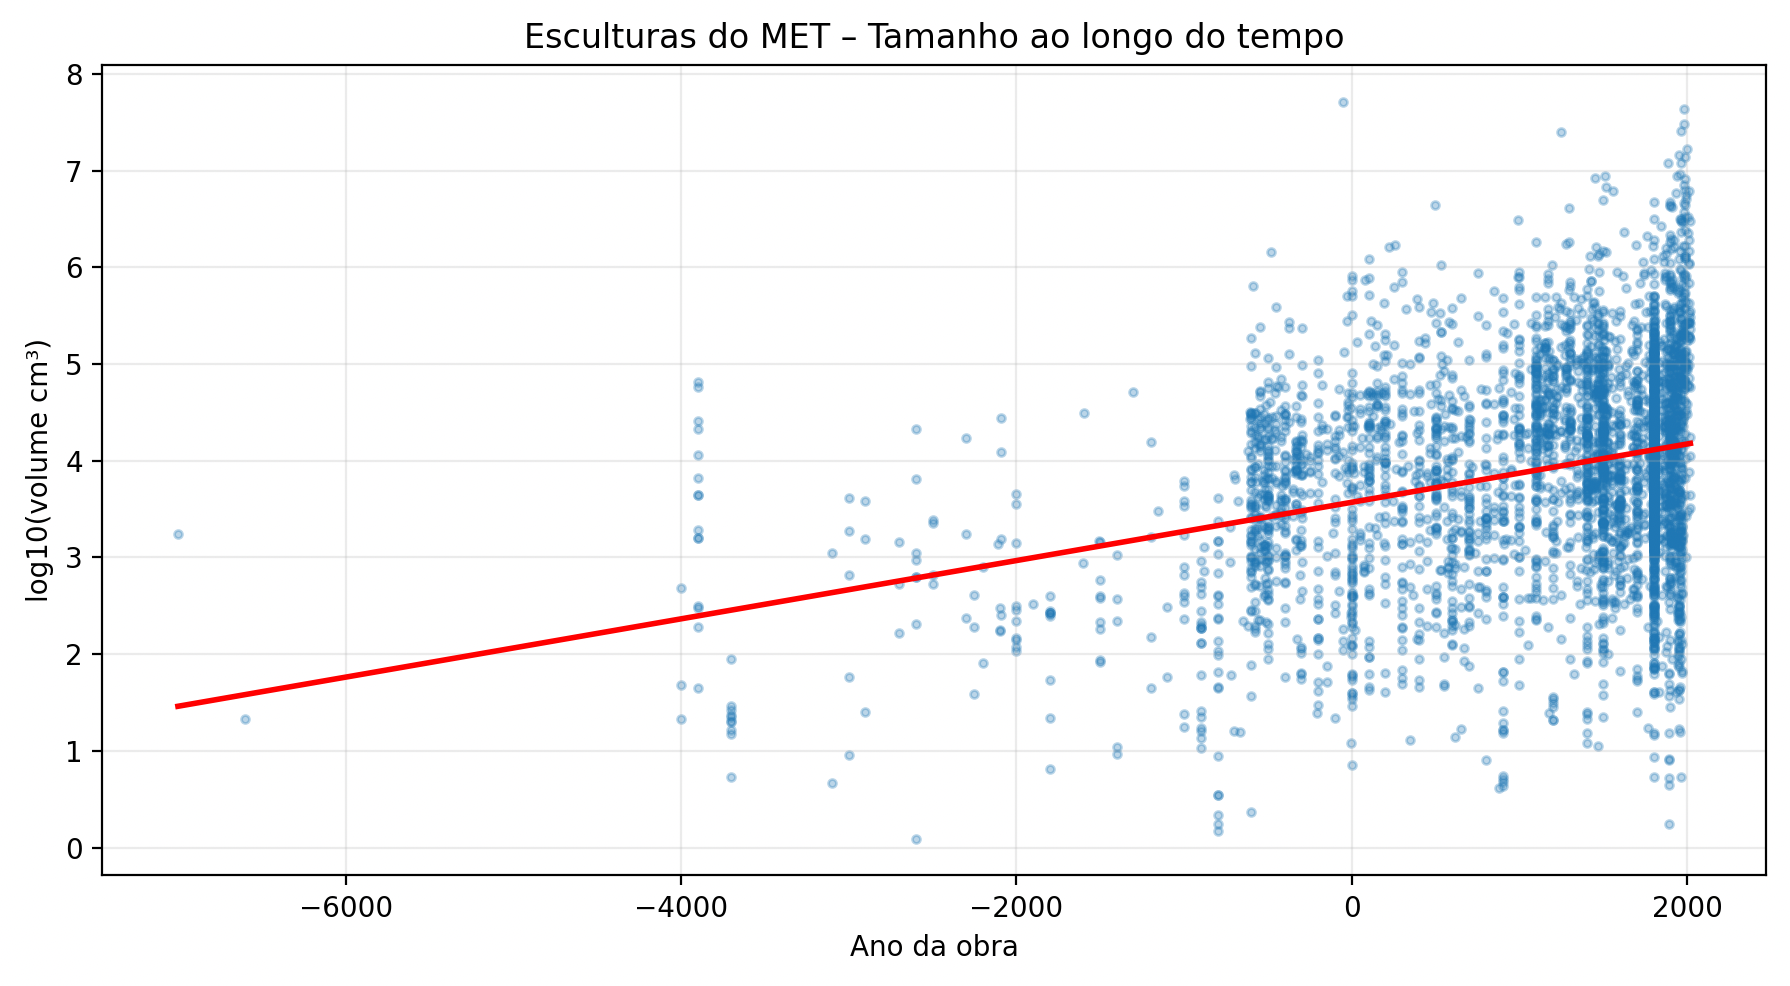
\includegraphics[width=0.8\textwidth]{../imagens/regressao_linear.png}
    \caption{Regressão linear do logaritmo do volume das esculturas em função do ano de confecção, mostrando tendência de aumento do tamanho ao longo do tempo.}
    \label{fig:regressao_linear}
\end{figure}

Os principais parâmetros estatísticos obtidos foram:
\begin{itemize}
    \item Intercepto $\beta_0 \approx 3,5703$
    \item Coeficiente $\beta_1$ (inclinação) $\approx 0,0003$
    \item Erro-padrão $\approx 1,5 \times 10^{-5}$
    \item Estatística t = 19,4
    \item p-valor < 0,0001
    \item R² ajustado = 0,084
\end{itemize}

Por conta do nível de significância de 5\% (adotado em todas as análises deste trabalho) e o p-valor quase nulo (< 0,0001), rejeitamos a hipótese nula com alta confiança. A estatística t de 19,4 reforça essa conclusão, indicando que o coeficiente estimado é 19,4 vezes maior que seu erro-padrão, ou seja, o coeficiente é estatisticamente significativo.

Porém, apesar desses resultados, o impacto prático do ano de confecção no volume das esculturas é pequeno. A Figura \ref{fig:regressao_linear} apresenta o diagrama de dispersão dos volumes (em escala log\textsubscript{10}) ao longo do tempo, com a reta de regressão ajustada: nota-se a inclinação positiva que confirma a tendência estatisticamente significativa, mas também um amplo espalhamento vertical dos pontos, sobretudo nos períodos mais recentes. Esse padrão visual reforça o R\textsuperscript{2} de apenas 8,4 \%, indicando que o tempo responde por uma fração muito pequena da variabilidade total — mais de 91 \% da variação decorre de fatores não contemplados neste modelo. Além disso, a inclinação ($\beta_1 \approx 0{,}0003$) mostra que, em média, mesmo ao longo de mil anos, o volume das esculturas tende apenas a duplicar, evidenciando que o efeito, embora real, é bastante pequeno e gradual.

\textbf{Resultado:} Rejeitamos H\textsubscript{0}. O teste mostra uma relação estatisticamente significativa entre o ano e o volume das esculturas, mas o efeito prático é consideravelmente pequeno. O R\textsuperscript{2} de 8,4\% confirma que o ano explica apenas uma pequena parte da variabilidade no tamanho das esculturas, sugerindo que outras variáveis como matéria-prima ou estilo artístico são muito mais significativas para o tamanho das esculturas no acervo do museu.

% Seção: Considerações Finais
\section{Considerações Finais}
As análises inferenciais tiveram como objetivo tentar identificar algumas das características que levam obras a serem colocadas em destaque no museu, explorando diversas variáveis em busca de explicações plausíveis para a alta exigência curatorial das obras destacadas (lembrando que estas contam apenas 3,85\% do total).

Considerando inicialmente somente os testes de hipótese apresentados com tamanho de amostra com 1.000 elementos aleatórios (para as hipóteses 1, 2 e 3), não houve evidência estatística, ao nível de 5\%, para rejeição da hipótese nula. Dessa forma, os testes não indicaram diferença estatisticamente significativa na área média das pinturas destacadas, na proporção de obras religiosas entre os destaques, nem correlação entre o ano de criação e o destaque.

Quanto à hipótese 4, explorada com todo o conjunto de dados, pudemos perceber que a regressão linear trouxe resultados estatisticamente significativos, mas de baixa influência prática.

Com base nas análises realizadas, observamos que a inferência estatística aplicada não identificou padrões determinísticos nos critérios de destaque curatorial do MET, o que sugere a necessidade de aprofundar investigações com novas variáveis ou fatores que possam indicar algum viés na seleção de obras destacadas.

Além disso, nossos experimentos serviram para mostrar o caráter inerentemente probabilístico de testes inferenciais, nos quais o nível de confiança, mesmo que alto, pode nos levar a conclusões estatisticamente corretas, mas que, populacionalmente, não se mostram verdadeiras. Esse fenômeno abre amplo espaço de discussão quanto às conclusões estatísticas, especialmente quando interpretadas fora do contexto técnico, onde há alto risco de confundir significância estatística com confirmação empírica absoluta.

Outro fator importante no contexto, como explorado com clareza na hipótese 1, é a influência do tamanho da amostra para realização de testes inferenciais, que deve ser mensurada com segurança para ter resultados com mais chance de se aproximar dos parâmetros populacionais.


\newpage
% Seção: Referências Bibliográficas
\section*{Referências Bibliográficas}
\begin{thebibliography}{99}
  \bibitem{ref1} The Metropolitan Museum of Art Open Access CSV. Disponível em: \url{https://github.com/metmuseum/openaccess}
  \bibitem{ref2} METROPOLITAN MUSEUM OF ART. Making the MET, 1870-2020. Disponível em: \url{https://www.metmuseum.org/exhibitions/listings/2020/making-the-met-1870-to-2020}
  \bibitem{ref3} METROPOLITAN MUSEUM OF ART. History of the Museum. Disponível em: \url{https://www.metmuseum.org/about-the-met/history}
\end{thebibliography}

% Anexos (ex.: sintaxe utilizada, código R, etc.)
\appendix
\section{Anexos}
% Insira os anexos, como códigos, aqui.

\subsection*{Código R: Tratamento de Dados}
\label{anx:codigo_data_treatment}
\begin{lstlisting}[language=R]
library(stringr) # For string manipulation (e.g., str_match, str_split, str_count)
library(dplyr)   # For data manipulation (e.g., mutate, select, rename)
library(tidyr)   # For data tidying (e.g., separate_rows)

# --- 1. Define the Dimension Parsing Function ---
# This function extracts and formats dimensions (e.g., "32.7 x 32.7" or "32.4 x 11.4 x 17.8")
parse_dimensions <- function(dim_string) {
  # Attempt to find dimensions in the format (NUM x NUM cm) or (NUM x NUM x NUM cm)
  pattern_combined <- "\\((\\d+\\.?\\d*)\\s*[x×]\\s*(\\d+\\.?\\d*)(?:\\s*[x×]\\s*(\\d+\\.?\\d*))?\\s*cm\\)"
  match_combined <- str_match(dim_string, pattern_combined)
  
  if (!is.na(match_combined[1, 1])) {
    # If a combined pattern is found, extract and format the numerical dimensions.
    dims <- na.omit(match_combined[1, 2:length(match_combined)])
    return(paste(dims, collapse = " x "))
  }
  
  # If no combined pattern, try to find individual (NUM cm) for H, W, D, etc.
  pattern_individual_cm <- "\\(\\s*(\\d+\\.?\\d*)\\s*cm\\)"
  all_individual_cm_matches <- str_extract_all(dim_string, pattern_individual_cm)[[1]]
  
  if (length(all_individual_cm_matches) > 0) {
    # Extract only the numbers from these matches.
    extracted_nums <- str_replace_all(all_individual_cm_matches, pattern_individual_cm, "\\1")
    # Take up to the first 3 dimensions (assuming H, W, D order for sculptures).
    extracted_nums <- head(extracted_nums, 3)
    return(paste(extracted_nums, collapse = " x "))
  }
  
  # If no relevant pattern is found, return NA.
  return(NA_character_)
}

# --- 2. Load the Original Dataset ---
# Ensure 'tabela_met.csv' is in your R working directory, or provide the full path.
# Example: tabela_met_original <- read.csv("C:/Users/YourUser/Documents/tabela_met.csv")
tabela_met_original <- read.csv("tabela_met.csv") %>%
  # Select only the required columns as they appear in the CSV (using backticks for names with dots).
  select(`Is.Highlight`, `Object.Begin.Date`, Tags, Dimensions) %>%
  # Rename columns for consistency (replacing dots with underscores, maintaining capitalization).
  rename(
    Is_Highlight = `Is.Highlight`,
    Object_Begin_Date = `Object.Begin.Date`
  )

# --- 3. Process Dimensions, Is_Sculpture, and Area/Volume for 'met_data' ---
# This block applies the dimension parsing, replaces the original column,
# adds the 'Is_Sculpture' binary flag, and calculates 'area/volume'.

met_data <- tabela_met_original %>%
  # Apply the parsing function to create a temporary 'parsed_dimensions' column.
  mutate(parsed_dimensions = sapply(Dimensions, parse_dimensions, USE.NAMES = FALSE)) %>%
  # Overwrite the original 'Dimensions' column with the parsed values.
  mutate(Dimensions = parsed_dimensions) %>%
  # Remove the temporary 'parsed_dimensions' column.
  select(-parsed_dimensions) %>%
  # Add the 'Is_Sculpture' column: TRUE if 3 dimensions (two 'x' separators), FALSE otherwise.
  # Handles NA values in 'Dimensions' by setting 'Is_Sculpture' to FALSE.
  mutate(
    Is_Sculpture = ifelse(
      is.na(Dimensions),
      FALSE,
      str_count(Dimensions, "x") == 2
    )
  ) %>%
  # Calculate 'area/volume': product of dimensions. NA if Dimensions is NA.
  mutate(
    `area/volume` = if_else(
      is.na(Dimensions),
      NA_real_, # Return numeric NA if Dimensions is NA.
      sapply(Dimensions, function(d_str) {
        # Split the dimension string into numeric values and calculate their product.
        dims_numeric <- as.numeric(str_split(d_str, " x ")[[1]])
        prod(dims_numeric)
      }, USE.NAMES = FALSE)
    )
  )

# --- 4. Expand 'Tags' Column for 'met_data_tags' ---
# This block takes the 'met_data' (which has the corrected Dimensions, etc.)
# and expands the 'Tags' column so each tag gets its own row.

met_data_tags <- met_data %>%
  # Split the 'Tags' column by the pipe '|' delimiter, creating new rows for each tag.
  # Handles cases where 'Tags' might be NA, producing NA in the expanded rows.
  separate_rows(Tags, sep = "\\|")

write.csv(met_data, "met_data.csv", row.names = FALSE)
write.csv(met_data_tags, "met_data_tags.csv", row.names = FALSE)

\end{lstlisting}

\subsection*{Código R: Criação da Variável 'Is\_Religious'}
\label{anx:codigo_creating_isReligious}
\begin{lstlisting}[language=R]
# Certifique-se de que os pacotes dplyr e stringr estão carregados
# Verifica e instala 'dplyr' se necessário, depois o carrega.
if (!requireNamespace("dplyr", quietly = TRUE)) {
  install.packages("dplyr")
}
library(dplyr)

# Verifica e instala 'stringr' se necessário, depois o carrega.
if (!requireNamespace("stringr", quietly = TRUE)) {
  install.packages("stringr")
}
library(stringr)

# --- Defina a lista de tags religiosas (REFINADA) ---
# Esta lista é usada para identificar se uma obra de arte tem um tema religioso,
# focando em figuras, conceitos e eventos diretamente religiosos.
religious_tags_list <- c(
  "Adoration of the Magi", "Adoration of the Shepherds", "Agony in the Garden",
  "Akshobhya", "Angels", "Annunciation", "Anubis", "Apostles", "Archangel Gabriel",
  "Assumption of the Virgin", "Baptism of Christ", "Bearing the Cross", "Bes",
  "Bible", "Bishops", "Bodhisattvas", "Brahma", "Buddha", "Buddhism",
  "Cain", "Cathedrals", "Ceremonial Objects", "Ceremony", "Chalices",
  "Chapels", "Christ", "Churches", "Circumcision", "Coptic",
  "Coronation of the Virgin", "Cross", "Croziers", "Crucifixion",
  "Daoism", "David", "Deities", "Demeter", "Demons", "Descent from the Cross",
  "Devil", "Doves", "Dragons", "Durga", "Evangelists", "Eve",
  "Flight Into Egypt", "Ganesha", "God the Father", "Goddess", "Gods",
  "Greek Mythology", "Hathor", "Hell", "Hera", "Herakles", "Hercules",
  "Hermes", "Herod", "Hinduism", "Holy Family", "Isis", "Jesus", "Joseph",
  "Judas", "Juno", "Jupiter", "Krishna", "Lamentation", "Last Judgement",
  "Last Supper", "Leda", "Lotuses", "Madonna", "Madonna and Child",
  "Maenads", "Maitreya", "Manjushri", "Marriage of the Virgin", "Mars",
  "Martin Luther", "Mary Magdalene", "Mercury", "Miter", "Monks", "Moses",
  "Mosques", "Mythical Creatures", "Mythology", "Nativity", "Nike", "Noah",
  "Nuns", "Pagodas", "Parables", "Parvati", "Pelicans", "Pilate", "Popes",
  "Praying", "Priests", "Queen of Sheba", "Radha", "Reliquaries", "Resurrection",
  "Ritual Objects", "Rosaries", "Saint Andrew", "Saint Anne", "Saint Anthony",
  "Saint Barbara", "Saint Bartholomew", "Saint Catherine", "Saint Christopher",
  "Saint Francis", "Saint George", "Saint Helena", "Saint Jerome", "Saint John",
  "Saint John the Baptist", "Saint John the Evangelist", "Saint Joseph",
  "Saint Lawrence", "Saint Leonard", "Saint Lucy", "Saint Luke", "Saint Mark",
  "Saint Matthew", "Saint Michael", "Saint Nicholas", "Saint Paul", "Saint Peter",
  "Saint Sebastian", "Saint Ursula", "Saint Zenobius", "Saints", "Shakyamuni",
  "Shepherds", "Shintō", "Shiva", "Sibyl", "Solomon", "Stupas", "Temples",
  "Virgin Mary", "Vishnu", "Visitation", "Zeus"
)

# --- Adicionar a coluna 'Is_Religious' ao seu dataframe 'met_data_religions' ---
# Este código deve ser inserido após todas as outras mutações para o dataframe original
# 'met_data' (como processamento de dimensões, is_sculpture, area/volume),
# mas antes de expandir as tags para 'met_data_tags'.

# Certifique-se de que 'met_data' está carregado ou foi gerado pelos passos anteriores.
# Exemplo (se estiver rodando este código isoladamente para teste):
# met_data <- data.frame(
#   ID = 1:5,
#   Tags = c("Circus|Musicians|Musical Instruments|Men|Women", "Birds", "Madonna|Jesus", NA, "Buddha|Monks"),
#   Is_Highlight = c(TRUE, FALSE, TRUE, FALSE, TRUE) # Exemplo de coluna Is_Highlight
# )


met_data_religions <- met_data %>%
  # Verifica se alguma das tags religiosas está presente na string 'Tags' para cada linha.
  # Constrói um padrão regex unindo todas as tags religiosas com '|' (OR).
  # 'ignore.case = TRUE' pode ser adicionado se a capitalização da tag variar.
  mutate(
    Is_Religious = ifelse(
      is.na(Tags), # Se a coluna Tags for NA, então não é religiosa
      FALSE,       # Caso contrário, defina como FALSE
      str_detect(Tags, paste(religious_tags_list, collapse = "|")) # Verifica se há correspondência
    )
  )

# Agora, 'met_data_religions' conterá o dataframe com a nova coluna 'Is_Religious'.
# Você pode verificar os resultados (opcional):
# print(head(met_data_religions))
\end{lstlisting}

\subsection*{Código R: Criação da Amostra para Teste de Proporção}
\label{anx:codigo_creating_sample_proportion}
\begin{lstlisting}[language=R]
# Certifique-se de que o pacote dplyr está carregado
library(dplyr)

# --- Gerar uma Amostra Aleatória ---
# Definindo o tamanho da amostra
sample_size <- 1000 # Exemplo: amostrar 1000 obras

# replace = FALSE` significa que cada linha é selecionada no máximo uma vez (amostragem sem reposição).
set.seed(123) # Um número qualquer, usado para reprodutibilidade
met_sample <- met_data %>%
  sample_n(size = sample_size, replace = FALSE)
\end{lstlisting}

\subsection*{Código R: Teste de Hipótese 2 (Proporção)}
\label{anx:codigo_testing_h2}
\begin{lstlisting}[language=R]
# Carrega o pacote dplyr para manipulação de dados
library(dplyr)

# Este script assume que 'met_sample' foi criado pelo bloco de código anterior.

# --- H2: Teste de Proporções ---
# H0: A proporção de obras com tema religioso entre os destaques é igual à dos não destacados.
# H1: A proporção de obras com tema religioso entre os destaques é diferente da dos não destacados.

# 1. Preparar os dados da AMOSTRA para o teste de proporções
# Contagem de obras religiosas e não religiosas para cada categoria de destaque NA AMOSTRA.
# Filtra linhas onde as colunas 'Is_Religious' ou 'Is_Highlight' são NA na amostra,
# pois elas são essenciais para o cálculo das proporções.
contingency_table_sample <- met_sample %>%
  filter(!is.na(Is_Religious) & !is.na(Is_Highlight)) %>%
  group_by(Is_Highlight) %>% # Agrupa os dados pela coluna 'Is_Highlight' (TRUE/FALSE)
  summarise(
    Religious_Count = sum(Is_Religious == TRUE),      # Conta o número de obras religiosas em cada grupo
    Non_Religious_Count = sum(Is_Religious == FALSE), # Conta o número de obras não religiosas em cada grupo
    Total_Count = n()                                 # Conta o total de obras em cada grupo
  )

# Extrair as contagens necessárias para a função prop.test()
# 'x' é um vetor com o número de "sucessos" (obras religiosas) para cada grupo (destacado/não destacado)
x_sample <- contingency_table_sample$Religious_Count
# 'n' é um vetor com o número total de observações para cada grupo
n_sample <- contingency_table_sample$Total_Count

# 2. Realizar o Teste de Proporções
# A função prop.test() é usada para comparar as proporções de dois ou mais grupos.
# x: vetor de contagens de sucessos.
# n: vetor de contagens totais (tamanho da amostra para cada grupo).
# alternative = "two.sided": indica um teste bicaudal (queremos saber se as proporções são diferentes,
#                             não se uma é especificamente maior ou menor que a outra).
# conf.level = 0.95: define o nível de confiança para o intervalo de confiança (95%).
proportion_test_result_sample <- prop.test(x = x_sample, n = n_sample, alternative = "two.sided", conf.level = 0.95)

# 3. Exibir os resultados
print("--- H2: Teste de Proporções (Tema Religioso vs. Destaque - Usando AMOSTRA) ---")
print("Tabela de Contingência (Contagens da Amostra):")
print(contingency_table_sample)
print("")
print("Resultado Completo do Teste de Proporções da Amostra:")
print(proportion_test_result_sample)

# 4. Interpretação do resultado
# Definir o nível de significância (alfa), geralmente 0.05.
alpha <- 0.05

print("")
print("--- Interpretação da Hipótese 2 (com Amostra) ---")
print(paste("Nível de Significância (alfa):", alpha))
print(paste("Valor-p calculado:", round(proportion_test_result_sample$p.value, 4)))

if (proportion_test_result_sample$p.value < alpha) {
  print("A decisão estatística é: Rejeitar a Hipótese Nula (H0).")
  print("Conclusão: Há evidências estatísticas significativas (com base nesta amostra) para afirmar que a proporção de obras com tema religioso entre os destaques é DIFERENTE da proporção entre as obras não destacadas na população.")
} else {
  print("A decisão estatística é: Não rejeitar a Hipótese Nula (H0).")
  print("Conclusão: Não há evidências estatísticas suficientes (com base nesta amostra) para afirmar que a proporção de obras com tema religioso difere significativamente entre os destaques e os não destacados na população.")
}

# Para entender as proporções em si:
prop_highlighted <- x_sample[contingency_table_sample$Is_Highlight == TRUE] / n_sample[contingency_table_sample$Is_Highlight == TRUE]
prop_non_highlighted <- x_sample[contingency_table_sample$Is_Highlight == FALSE] / n_sample[contingency_table_sample$Is_Highlight == FALSE]

print(paste("\nProporção de obras religiosas entre as destacadas (na amostra):", round(prop_highlighted, 4)))
print(paste("Proporção de obras religiosas entre as não destacadas (na amostra):", round(prop_non_highlighted, 4)))
\end{lstlisting}

\subsection*{Código Python: Análise de Estatísticas Descritivas}
\label{anx:codigo_estatisticas_descritivas}
\begin{lstlisting}[language=Python]
import pandas as pd

# ======================================================
# Leitura dos Arquivos

data = pd.read_csv("met_data.csv")
data_tags = pd.read_csv("met_data_tags.csv")

data_pinturas = data[data["Is_Sculpture"] == False]  # dados das pinturas
data_esculturas = data[data["Is_Sculpture"] == True]  # dados das esculturas

# ======================================================
# Estatisticas Descritivas por Variavel

# ------------------------------------------------------
# 1. Ano da Obra

anos = data["Object_Begin_Date"]

media_ano = anos.mean()
mediana_ano = anos.median()
desvio_ano = anos.std()
min_ano = anos.min()
max_ano = anos.max()

print("Ano das obras:")
print(f"Média: {media_ano:.2f}")
print(f"Mediana: {mediana_ano}")
print(f"Desvio padrão: {desvio_ano:.2f}")
print(f"Mínimo: {min_ano}, Máximo: {max_ano}")

# ------------------------------------------------------
# 2. Area das Pinturas

areas = data_pinturas["area/volume"]

media_area = areas.mean()
mediana_area = areas.median()
desvio_area = areas.std()
min_area = areas.min()
max_area = areas.max()

print("\nÁrea das pinturas:")
print(f"Média: {media_area:.2f}")
print(f"Mediana: {mediana_area}")
print(f"Desvio padrão: {desvio_area:.2f}")
print(f"Mínimo: {min_area}, Máximo: {max_area}")

# ------------------------------------------------------
# 3. Volume das Esculturas

volumes = data_esculturas['area/volume']

media_volume = volumes.mean()
mediana_volume = volumes.median()
desvio_volume = volumes.std()
min_volume = volumes.min()
max_volume = volumes.max()

print("\nVolume das esculturas:")
print(f"Média: {media_volume:.2f}")
print(f"Mediana: {mediana_volume}")
print(f"Desvio padrão: {desvio_volume:.2f}")
print(f"Mínimo: {min_volume}, Máximo: {max_volume}")

# ------------------------------------------------------
# 4. Tags

frequencia_tags = data_tags["Tags"].value_counts()
print("\nTags mais frequentes:")
print(frequencia_tags.head(10).to_string())  # 10 mais comuns

# ------------------------------------------------------
# 5. Obras em Destaque

n_total = len(data)
n_destaques = data["Is_Highlight"].sum()
proporcao = n_destaques / n_total

print("\nProporção de obras em destaque:")
print(f"Total de obras: {n_total}")
print(f"Número de destaques: {n_destaques}")
print(f"Proporção: {proporcao:.4f} ({proporcao*100:.2f}%)")
\end{lstlisting}

\subsection*{Código Python: Teste de Hipótese 1 (Média)}
\label{anx:codigo_hipotese1}
\begin{lstlisting}[language=Python]
import pandas as pd
from scipy.stats import ttest_ind

# ======================================================
# Preparacao dos Dados

# ------------------------------------------------------
# 1. Extracao

data = pd.read_csv("../data/met_data.csv")
data_pinturas = data[data["Is_Sculpture"] == False]  # dados das pinturas


# ------------------------------------------------------
# 2. Criacao de Amostra Aleatria (1000 pinturas)

amostra = data_pinturas.sample(n = 1000, random_state=123)  # random_state eh usado pra gerar a mesma amostra
# o tamanho da amostra e random_state podem ser modificados como desejado

# ------------------------------------------------------
# 3. Filtro de Colunas Relevantes e Remocao de NanNs

amostra = amostra[["Is_Highlight", "area/volume"]].dropna()

# ------------------------------------------------------
# 4. Separacao de Obras Destacadas e Nao Destacadas

destacadas = amostra[amostra["Is_Highlight"] == True]["area/volume"]
nao_destacadas = amostra[amostra["Is_Highlight"] == False]["area/volume"]

# ======================================================
# Exploracao das Hipoteses
'''
H0: A média da área das pinturas destacadas é igual à das não destacadas.
H1: As médias são diferentes.
'''

print("Hipótese 1 — Teste de comparação de médias (área das pinturas)\n")

# ------------------------------------------------------
# 1. Calculo das Medias

media_destacadas = destacadas.mean()
media_nao_destacadas = nao_destacadas.mean()

# ------------------------------------------------------
# 2. Teste t de Student (Para Amostras Independentes)

t, p_valor = ttest_ind(destacadas, nao_destacadas)

print(f"Média das áreas (destacadas): {media_destacadas:.2f}")
print(f"Média das áreas (não destacadas): {media_nao_destacadas:.2f}\n")
print(f"t = {t:.4f}")
print(f"p-valor = {p_valor:.4f}\n")

# ------------------------------------------------------
# 3. Validacao da Hipotese

a = 0.05
if p_valor < a:
    print("Rejeitamos H0: Há diferença significativa entre as médias.")
else:
    print("Não rejeitamos H0: Não há diferença significativa entre as médias.")
\end{lstlisting}

\subsection*{Código Python: Teste de Hipótese 3 (Correlação)}
\label{anx:codigo_hipotese3}
\begin{lstlisting}[language=Python]
import pandas as pd                  
from scipy.stats import pointbiserialr 
import numpy as np                    
import matplotlib.pyplot as plt

# ------------------------------------------------------
# 1. PREPARAÇÃO DOS DADOS

data = pd.read_csv("../data/met_data.csv")

amostra = data.sample(
    n=1000,                           
    random_state=123
)

# POPULAÇÃO:
# Mantém só as colunas de interesse e remove linhas com NaN
populacao = data[["Object_Begin_Date", "Is_Highlight"]].dropna()
# Converte o booleano em inteiro 1/0
populacao["Highlight_Num"] = populacao["Is_Highlight"].astype(int)

# AMOSTRA:
# Seleciona apenas as colunas de interesse, e remove linhas com valores não disponíveis
amostra = amostra[["Object_Begin_Date", "Is_Highlight"]].dropna()
# Transforma o booleano True/False de 'Is_Highlight' em inteiro 1/0
amostra["Highlight_Num"] = amostra["Is_Highlight"].astype(int)

# ------------------------------------------------------
# 2. FORMULAÇÃO DAS HIPÓTESES

# H0: rho_pb = 0 (nenhuma correlação entre Object_Begin_Date e Highlight_Num)
# H1: rho_pb != 0 (existe correlação)

# ------------------------------------------------------
# 3. CÁLCULO DO COEFICIENTE POINT-BISERIAL

# POPULAÇÃO
rho_pb_populacao, p_valor_populacao = pointbiserialr(
    populacao["Highlight_Num"],
    populacao["Object_Begin_Date"]
)

# AMOSTRA
# Chama pointbiserialr com as duas colunas de interesse da amostra, e retorna o valor do coeficiente de correlação em rho_pb (rho point-biserial), e retorna p-valor, que indica a significância estatística. O p-valor diz o quão improvável seria obter no caso de nenhuma correlação (H0 correta)
rho_pb_amostra, p_valor_amostra = pointbiserialr(
    amostra["Highlight_Num"], 
    amostra["Object_Begin_Date"]
)


print("\nPoint-Biserial Correlation (Object_Begin_Date and Is_Highlight):\n")

# POPULAÇÃO
print("População:")
print(f"rho_pb_populacao = {rho_pb_populacao:.4f}") 
print(f"p-valor_populacao = {p_valor_populacao:.4f}\n") 

# AMOSTRA
print("Amostra:")
print(f"rho_pb_amostra = {rho_pb_amostra:.4f}") 
print(f"p-valor_amostra = {p_valor_amostra:.4f}\n")  

# ------------------------------------------------------
# 4. INTERPRETAÇÃO

# Define o nível de significância (5%)
alpha = 0.05                     

print("\nINTERPRETAÇÃO DOS RESULTADOS:\n")

# POPULAÇÃO
print("População:")
if p_valor_populacao < alpha:
    sentido = "positiva" if rho_pb_populacao > 0 else "negativa"
    print(f"Rejeitamos H0, pois há correlação {sentido} significativa.")
else:
    print("Não rejeitamos H0: nenhuma correlação significativa.")

# AMOSTRA
print("\nAmostra:")
if p_valor_amostra < alpha: 
    sentido = "positiva" if rho_pb_amostra > 0 else "negativa"
    print(f"Rejeitamos H0, pois há correlação {sentido} significativa.")
else:
    print("Não rejeitamos H0: nenhuma correlação significativa.")

# ------------------------------------------------------
# 5. VISUALIZAÇÃO

# POPULACAO
plt.figure(figsize=(10,6))
y = populacao["Highlight_Num"] + (np.random.rand(len(populacao)) - 0.5) * 0.1
plt.scatter(populacao["Object_Begin_Date"], y, alpha=0.4)
plt.yticks([0,1], ["Não-Highlight","Highlight"])
plt.xlabel("Ano de Início da Obra")
plt.title("Object_Begin_Date e Is_Highlight")
plt.tight_layout()           
plt.show()        

# AMOSTRA
plt.figure(figsize=(10,6))
y = amostra["Highlight_Num"] + (np.random.rand(len(amostra)) - 0.5) * 0.1
plt.scatter(amostra["Object_Begin_Date"], y, alpha=0.4)
plt.yticks([0,1], ["Não-Highlight","Highlight"])
plt.xlabel("Ano de Início da Obra")
plt.title("Object_Begin_Date e Is_Highlight")
plt.tight_layout()           
plt.show()                   
\end{lstlisting}

\subsection*{Código Python: Teste de Hipótese 4 (Regressão Linear)}
\label{anx:codigo_hipotese4}
\begin{lstlisting}[language=Python]
import pandas as pd
import numpy as np
import sys
import statsmodels.formula.api as smf
import matplotlib.pyplot as plt
from pathlib import Path

csv = sys.argv[1] if len(sys.argv) > 1 else "trabalho 2/data/met_data.csv"
if not Path(csv).is_file():
    sys.exit(f"Arquivo não encontrado: {csv}")

# 1. carregar e padronizar nomes
df = pd.read_csv(csv)
df.columns = (df.columns.str.strip()
                        .str.lower()
                        .str.replace(r"[^\w]+", "_", regex=True))

# 2. filtrar esculturas válidas
esc = (df.query("is_sculpture == True")
         .dropna(subset=["object_begin_date", "area_volume"])
         .copy())

# 3. log10 do volume
esc["log_vol"] = np.log10(esc.area_volume.replace(0, np.nan))
esc = esc.dropna(subset=["log_vol"])      # garante mesmas linhas no gráfico e modelo

# 4. regressão
model = smf.ols("log_vol ~ object_begin_date", data=esc).fit()
print("\n--------  Esculturas – Regressão log(volume) ~ ano  --------")
print(model.summary())

# 5. plota o gráfico
plt.figure(figsize=(9,5))
plt.scatter(esc.object_begin_date, esc.log_vol, s=8, alpha=.3)
x = np.linspace(esc.object_begin_date.min(), esc.object_begin_date.max(), 200)
y = model.params.Intercept + model.params.object_begin_date * x
plt.plot(x, y, c="red", lw=2)
plt.xlabel("Ano da obra")
plt.ylabel("log10(volume cm3)")
plt.title("Esculturas do MET – Tamanho ao longo do tempo")
plt.grid(alpha=.25)
plt.tight_layout()
plt.show()
\end{lstlisting}

\end{document}